\documentclass[10pt,a4paper]{article}
\usepackage[utf8]{inputenc}
\usepackage[parfill]{parskip}
\usepackage[section]{placeins}
\usepackage{subfig}
\usepackage{graphicx}
\usepackage{array}
\usepackage{tabularx}
\usepackage[scientific-notation=true]{siunitx}
\usepackage{amsmath}

\author{Dominik Nerger (i6146759)}
\title{Text Mining South Park}
\date{\today}

\begin{document}
	\maketitle
	
	\tableofcontents
	
	\section{Introduction}
	
	This report is part of the second assignment for the course Computer Vision and focusses on face recognition using Principal Component Analysis and k-nearest neighbors classification.
	
	\section{Data set}
	\begin{figure}[h]
	\centering
	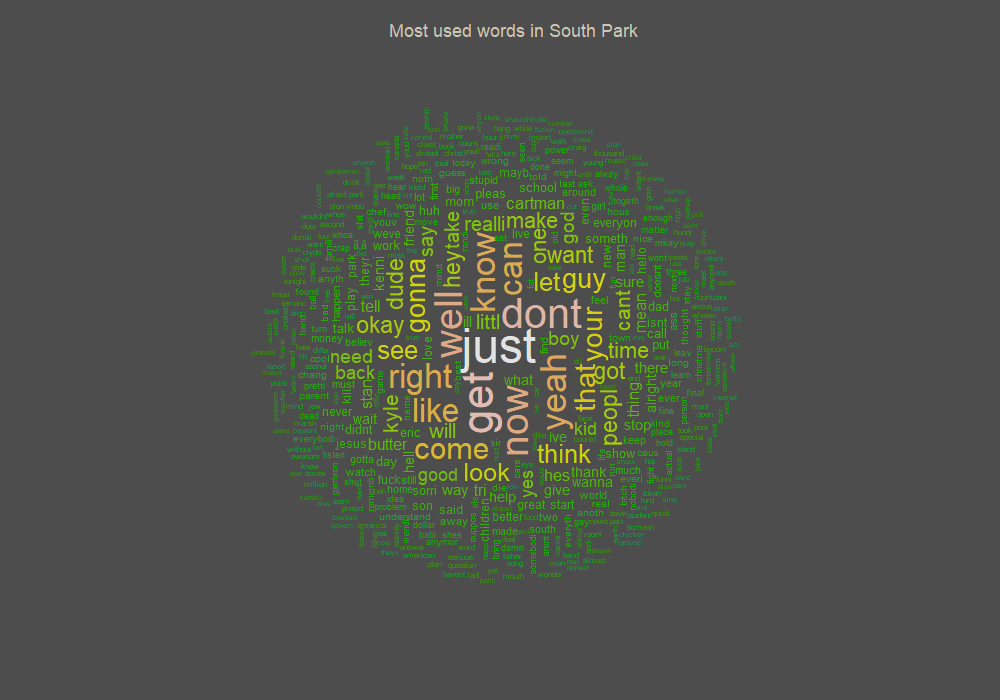
\includegraphics[scale=0.9]{images/WordCloud.png}
	\caption{General wordcloud, containing terms by frequency}
	\label{fig:WordCloud}
	\end{figure}
	
	\begin{figure}[h]
	\centering
	\includegraphics[scale=0.9]{images/WordCloud-TFIDF.png}
	\caption{General wordcloud, containing terms by TF-IDF score}
	\label{fig:WordCloud-TFIDF}
	\end{figure}
	\begin{figure}[h]
	\centering
	\includegraphics[scale=0.9]{images/WordCloud-TFIDF.png}
	\caption{Wordcloud containing ngrams (n=4) by frequency}
	\label{fig:WordCloud-ngram}
	\end{figure}
	
	\begin{figure}[h]
	\centering
	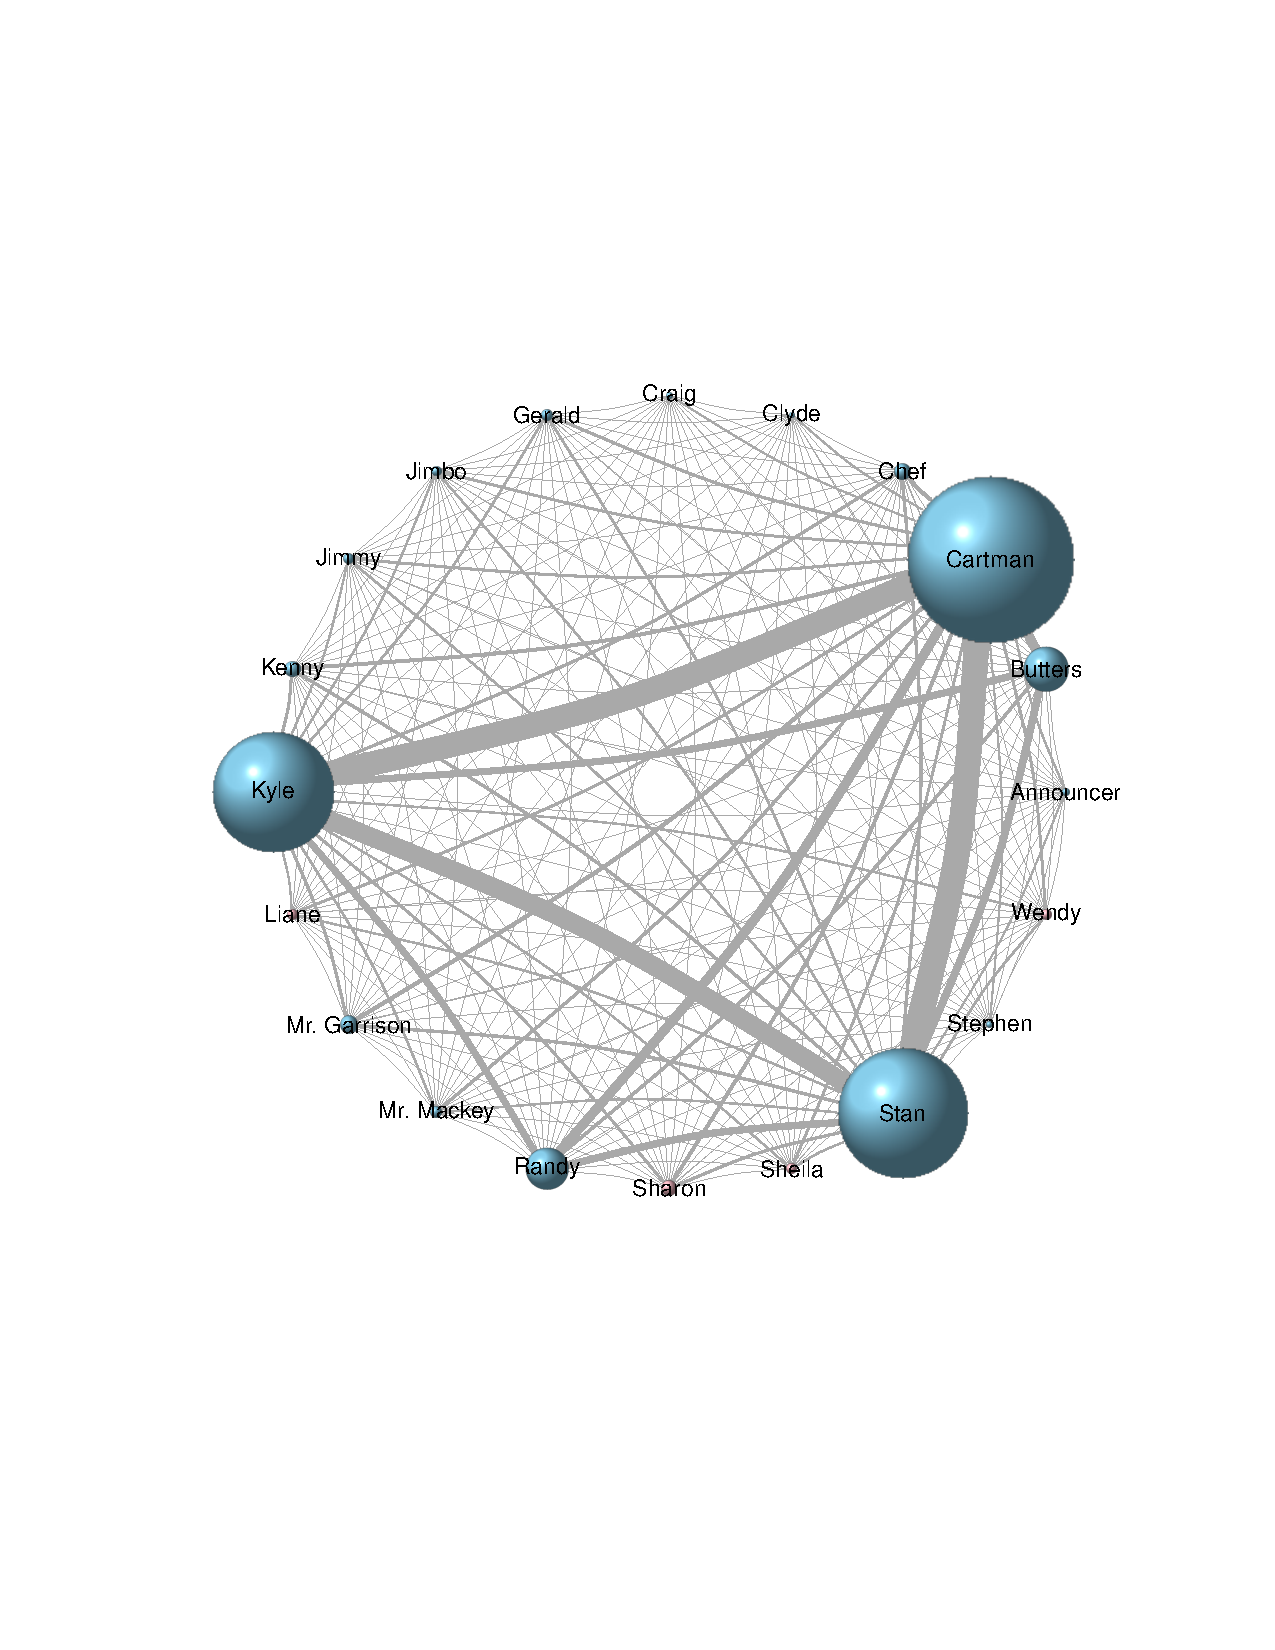
\includegraphics[scale=0.7]{images/CoOccurence Matrix.pdf}
	\caption{Wordcloud containing ngrams (n=4) by frequency}
	\label{fig:CoOccurence}
	\end{figure}
	
	\section{Pre-processing}
	
	
	\section{Implementation and results}
	
	
	\section{Conclusion}
	In conclusion, 

	\section{Future work}
\end{document}
